\chapter{MÉTODO DE VOLÚMENES FINITOS Y ESQUEMA DE ROE}
A continuación se describen el método y los esquemas a utilizar para llevar a cabo una solución numérica de una ecuación de conservación. La idea principal del capítulo es describir el método de volúmenes finitos y la motivación de su uso. Se explicarán los esquemas adecuados para aplicar el mencionado método, un solucionador del problema de Riemann, denominado esquema de Godunov y otro solucionador aproximado del problema de Riemann, denominado esquema de Roe. Este último es el esquema elegido para resolver las ecuaciones de Euler en este texto.\\
El contenido de este capítulo se basa en la parte \textit{Numerical Methods} del texto \cite{Leveque} de Randall LeVeque.

\section{Método de volúmenes finitos}
El método de volúmenes finitos (MVF) es un método numérico de integración que se especializa en resolver ecuaciones diferenciales escritas en forma conservativa. El MVF destaca por ofrecer una interpretación peculiar de la función a resolver, ya que es un método basado en la forma \textbf{integral} de las ecuaciones.
\subsection{Discretización del problema}
Al aplicar un método numérico para resolver una ecuación diferencial se necesita discretizar el dominio de la función y la función misma. Considerando a  $D = [a,b]$ como el dominio espacial de la solución de una ecuación de conservación, para aplicar el MVF este dominio se divide en $N$ intervalos iguales llamado \textbf{celdas}. Cada celda se denomina $\mathcal{C}_i$ y se define como un intervalo, $\mathcal{C}_i = [x_i, x_{i+1}]$. Además, cada celta tiene un ancho $h$, dado por
\begin{equation}
	h = \frac{b-a}{N}
\end{equation}
\begin{figure}[ht]
	\centering
	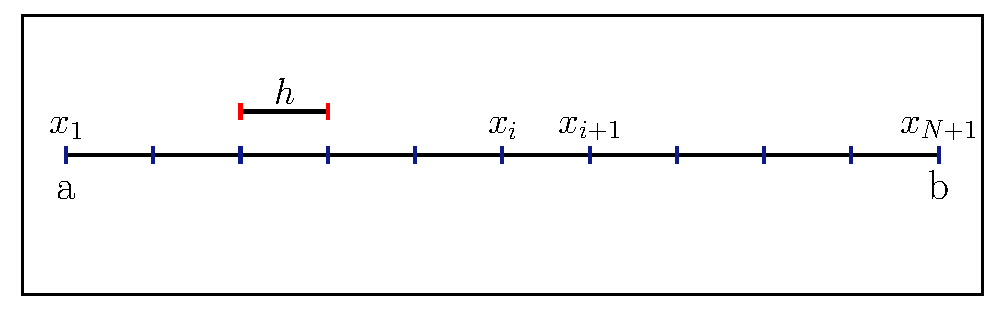
\includegraphics[width=\linewidth]{../some_plots/cap2/graficas/domain.pdf}
	\label{fig:discretizacion-eje-x}
	\caption{Esquema de símbolos usados para la discretización del dominio espacial. \textbf{Fuente:} elaboración propia.}
\end{figure}


